\documentclass[times, utf8, diplomski, numeric]{fer}
\usepackage{booktabs}
\usepackage{listings}
\usepackage{color}
\usepackage{pdfpages}



\definecolor{lightgray}{rgb}{.9,.9,.9}
\definecolor{darkgray}{rgb}{.4,.4,.4}
\definecolor{purple}{rgb}{0.65, 0.12, 0.82}

\definecolor{mygreen}{rgb}{0,0.6,0}
\definecolor{mygray}{rgb}{0.5,0.5,0.5}
\definecolor{mymauve}{rgb}{0.58,0,0.82}

\lstset{ %
    backgroundcolor=\color{white}, % choose the background color; you must add \usepackage{color} or \usepackage{xcolor}
    basicstyle=\footnotesize, % the size of the fonts that are used for the code
    breakatwhitespace=false, % sets if automatic breaks should only happen at whitespace
    breaklines=true, % sets automatic line breaking
    captionpos=b, % sets the caption-position to bottom
    commentstyle=\color{mygreen}, % comment style
    deletekeywords={...}, % if you want to delete keywords from the given language
    escapeinside={\%*}{*)}, % if you want to add LaTeX within your code
    extendedchars=true, % lets you use non-ASCII characters; for 8-bits encodings only, does not work with UTF-8
    frame=single, % adds a frame around the code
    keepspaces=true, % keeps spaces in text, useful for keeping indentation of code (possibly needs columns=flexible)
    keywordstyle=\color{blue}, % keyword style
    % language=Octave, % the language of the code
    morekeywords={*,...}, % if you want to add more keywords to the set
    numbers=left, % where to put the line-numbers; possible values are (none, left, right)
    numbersep=5pt, % how far the line-numbers are from the code
    numberstyle=\tiny\color{mygray}, % the style that is used for the line-numbers
    rulecolor=\color{black}, % if not set, the frame-color may be changed on line-breaks within not-black text (e.g. comments (green here))
    showspaces=false, % show spaces everywhere adding particular underscores; it overrides 'showstringspaces'
    showstringspaces=false, % underline spaces within strings only
    showtabs=false, % show tabs within strings adding particular underscores
    stepnumber=1, % the step between two line-numbers. If it's 1, each line will be numbered
    stringstyle=\color{mymauve}, % string literal style
    tabsize=2, % sets default tabsize to 2 spaces
    title=\lstname % show the filename of files included with \lstinputlisting; also try caption instead of title
}
%END of listing package%
 
%define JavaScript language
\lstdefinelanguage{JavaScript}{
    keywords={typeof, new, true, false, function, null, var, in, of, let, const, class, extends, implements, constructor, super, this, async, interface, type, declare, module},
    keywordstyle=\color{blue}\bfseries,  % blue % black
    ndkeywords={import, from, as, export, default, return, if, for, switch, while, do, else, case, break, continue, await, try, catch},
    ndkeywordstyle=\color{purple}\bfseries,  % purple % black
    identifierstyle=\color{black},
    sensitive=false,
    comment=[l]{//},
    morecomment=[s]{/*}{*/},
    commentstyle=\color{mygreen}\ttfamily,  % green % mygray
    stringstyle=\color{red}\ttfamily,  % red % darkgray
    morestring=[b]',
    morestring=[b]",
    morestring=[b]`,
}
 
\lstset{
    language=JavaScript,
    extendedchars=true,
    basicstyle=\footnotesize\ttfamily,
    showstringspaces=false,
    showspaces=false,
    numbers=left,
    numberstyle=\footnotesize,
    numbersep=9pt,
    tabsize=2,
    breaklines=true,
    showtabs=false,
    captionpos=b
}

\renewcommand{\lstlistingname}{Isječak koda}
\renewcommand{\lstlistlistingname}{Popis isječaka koda}

\newcommand{\razmakp}{\vspace{18pt}}
\newcommand{\razmaks}{\vspace{10pt}}
\newcommand{\uvlakas}{\hspace{0.5cm}}



\begin{document}

\thesisnumber{1937}

\title{Sustav za podršku učenju koncepata deklarativne programske paradigme}

\author{Petar Kovačević}

\maketitle

% Ispis stranice s napomenom o umetanju izvornika rada. Uklonite naredbu \izvornik ako želite izbaciti tu stranicu.
\izvornik

% Dodavanje zahvale ili prazne stranice. Ako ne želite dodati zahvalu, naredbu ostavite radi prazne stranice.
\zahvala{}

\tableofcontents



% Uvod
\chapter{Uvod}

TODO



% Tehnologije
\chapter{Tehnologije}


% Jezik
\section{Jezik}

Programski jezici implementacije sustava su JavaScript za poslužiteljsku stranu \engl{sever-side} i TypeScript za aplikacijsku, odnosno klijentsku stranu \engl{client-side}.
Na klijentskoj strani je u velikoj mjeri prisutna JSX, odnosno TSX sintaksa.

% JavaScript (ECMAScript)
\subsection{JavaScript (ECMAScript)}

JavaScript je viši programski jezik opće namjene koji se primarno izvodi u internet preglednicima, odnosno uz HTML i CSS (koji nisu jezici opće namjene) jedini je programski jezik kojeg preglednici nativno (bez dodataka) podržavaju.
Sintaksa jezika je slična ostalim jezicima takozvane C obitelji jezika, ali za razliku od njih riječ je o dinamičko-tipiziranom \engl{dynamicly typed} interpretabilnom jeziku.\citep{mdn_js}

Jezik podržava više paradigmi, ali je primarno objektno orijentiran i to, za razliku od drugih popularnih jezika te skupine, baziran na prototipovima \engl{prototype-based}, a ne na razredima.
Ključna razlika između ta dva pristupa je u implementaciji nasljeđivanja. U JavaScript-u se nasljeđivanje odvija proširivanjem \emph{prototipova} koji su posebni tipovi objekata pomoću kojih se stvaraju objekti.\citep{wiki_proto_prog}
Budući da je koncept prototipova većini programera stran i da, zbog dinamičnih tipova u JavaScriptu, neoprezno korištenje može dovesti do nepredviđenih grešaka, od verzije ECMAScript 2015\footnote{
    također poznata pod nazivom ECMAScript 6, skraćeno ES6
} dodani su razredi kao sintaksni šećer \engl{syntax sugar} koje programeri mogu koristiti slično drugim objektno orijentiranim jezicima, a transpilatori\footnote{
    kompilatori, odnosno jezični prevoditelji koji prevode novije verzije JavaScript jezika u starije kako bi stariji preglednici mogli izvršavati napisan kod, primjer: Babel (\url{https://babeljs.io})
} ih prevode u prototipove\citep{mdn_class}.

\razmakp

ECMAScript je pojam koji se često koristi kao alternativno ime za jezik JavaScript, posebice kada se želi naglasiti korištenje modernih novijih verzija jezika.
ECMAScript je ustvari specifikacija skriptnog jezika pod kodovima ECMA-262 i ISO/IEC 16262 kojeg održava međunarodna organizacija Ecma International\footnote{\url{https://www.ecma-international.org}}.
Taj standard implementira više programskih jezika, ali je daleko najpoznatiji JavaScript za kojeg je primarno standard i napisan.
U trenutku pisanja ovog rada najnovija verzija standarda je verzija 9, odnosno ECMAScript 2018.\citep{wiki_es}

\razmakp
% Asinkronost i Promise objekt
\subsubsection{Asinkronost i \emph{Promise} objekt} \label{sec:async}

Ključan detalj za JavaScript i jezike koje se prevode u JavaScript je da se izvode u jednodretvenom okruženju i da je konkurentnost tog okruženja bazirana na modelu petlje događaja \engl{event loop}.
Pojednostavljena verzija tog modela je da za svaki asinkroni događaj (primjerice dohvat podataka s poslužitelja) postoji funkcija povratnog poziva \engl{callback function} i ta funkcija se stavlja u red poruka \engl{message queue}.
Dretva u kojem se izvršava JavaScript kod je ostvarena kao neblokirajuća beskonačna petlja koja, u trenutku kada ne izvršava neki dio koda, provjerava red poruka.
Ako je asinkron događaj elementa izvađenog iz reda gotov, petlja izvršava funkciju povratnog poziva, inače stavlja događaj nazad u red i provjerava idući element reda.\citep{mdn_event_loop}

\razmakp

U praksi se pokazalo da aplikacijska logika često zahtijeva da se neki asinkron događaj poziva nakon drugog asinkronog događaja, odnosno unutar funkcije povratnog poziva prvog događaja bi se pozivao događaj sa svojom funkcijom povratnog poziva.
Ovakav scenarij se često mogao ponoviti i u toj unutarnjoj funkciji povratnog poziva što bi dovelo do teško održivog i teško čitljivog koda kojeg neki programeri zovu „callback hell“ ili „callback pyramid of doom“.

\razmakp % Primjer ugnježđivanja funkcija povratnog poziva
\begin{lstlisting}[language=JavaScript, caption={Primjer ugnježđivanja funkcija povratnog poziva}, label={lst:callback}]
doSomething(function(result) {
  doSomethingElse(result, function(newResult) {
    doAnotherThing(newResult, function(finalResult) {
      console.log('Got the final result: ' + finalResult);
    }, failureCallback);
  }, failureCallback);
}, failureCallback);
\end{lstlisting}
\razmaks

Rješenje za taj problem je došlo u ECMAScript 2015 uvođenjem \emph{Promise} objekta.
\emph{Promise} je poseban tip objekta koji jer reprezentacija nekog asinkronog događaja, odnosno omotava funkciju povratnog poziva tog asinkronog događaja.
Funkcija je omotana u \emph{obećanje} da će se izvršiti i nad tim objektom može se pozivom metode \emph{then} nizati daljnja \emph{obećanja} asinkronih događaja, odnosno definirati što se izvršava nakon uspješnog ili neuspješnog (metoda \emph{catch}) izvršavanja funkcije povratnog poziva.

\razmakp % Primjer korištenja Promise objekta
\begin{lstlisting}[language=JavaScript, caption={Primjer korištenja \emph{Promise} objekta}, label={lst:promise}]
doSomething()
.then(function(result) {
  return doSomethingElse(result);
})
.then(function(newResult) {
  return doAnotherThing(newResult);
})
.then(function(finalResult) {
  console.log('Got the final result: ' + finalResult);
})
.catch(failureCallback);
\end{lstlisting}
\razmaks

Metode \emph{then} i \emph{catch} su nužne jer \emph{Promise} omotava asinkrone operacije i ne može se izravno iz njega iščitati rezultat operacije jer se u trenutku izvršavanja koda ne zna u kojem je stanju \emph{Promise} objekt.

\begin{figure}[!htb] % Životni ciklus Promise objekta
    \centering
    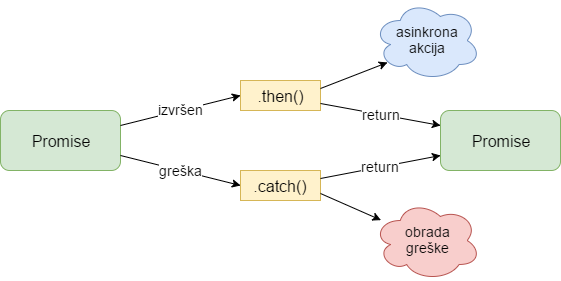
\includegraphics[width=14cm]{images/promise.png}
    \caption{Životni ciklus \emph{Promise} objekta}
    \label{fig:promise_lifecycle}
\end{figure}

\emph{Promise} u svom životnom ciklusu prolazi kroz dva od tri moguća stanja.
Na početku je u pripravnosti \engl{pending} i ovisno o uspješnosti asinkrone operacije odlazi u stanje \emph{ispunjen} \engl{fulfilled} ili \emph{odbijen} \engl{rejected} (vidi sliku \ref{fig:promise_lifecycle}).
U trenutku ulaska u jedno od dva konačna stanja poziva se funkcija ili novi \emph{Promise} definiran kao rezultat funkcije koja je argument \emph{then} ili \emph{catch} metode.
U slučaju da \emph{Promise} uđe u odbijeno stanje, a nema poziva \emph{catch} metode, u aplikaciji će se propagirati greška da odbijeno stanje nije obrađeno \engl{unhandled promise rejection}.\citep{mdn_promise}

\razmakp

Budući da novi koncept \emph{Promise} objekta nije u savršeno pomogao s čitljivošću koda, pogotovo u situacijama kada je nužno obraditi grešku u sredini nekog većeg lanca \emph{Promise} objekata, u specifikaciji ECMAScript 2017 se dodatno uljepšala sintaksa korištenja \emph{Promise} objekata uvođenjem novih ključnih riječi \emph{async} i \emph{await} koji se mogu kombinirati s postojećom \emph{try} i \emph{catch} sintaksom.
Ideja je da se funkcije koje su asinkrone, odnosno vraćaju \emph{Promise} označe ključnom riječi \emph{async}.
Rezultat te funkcije se može odmotati korištenjem ključne riječi \emph{await}.
Time se postiže neblokirajuće čekanje na izvršavanje asinkrone operacije, ekvivalentno tome da se pozvalo \emph{then}\footnote{
    Transpilator u praksi ne prevodi \emph{await} i kod koji slijedi u \emph{then} već prevodi cijelu \emph{async} funkciju u funkciju generator \engl{generator function} gdje samo \emph{await} zamjeni s \emph{yield“} Ta funkcija generator je potom omotana u drugu funkciju koja koristi taj generator da bi iterirala po koracima lanca asinkronih operacija i pozvala \emph{then} za idući dio lanca. Nakon toga je funkcija generator, budući da je i ona relativno novi dodatak (ECMAScript 2015), prevedena u kod koji je u skladu sa starijim standardom.
}.
Za obradu grešaka, umjesto \emph{catch} metode koristi se postojeći \emph{catch} blok.

\razmakp % Primjer korištenja ECMAScript 2017 sintakse
\begin{lstlisting}[language=JavaScript, caption={Primjer korištenja ECMAScript 2017 sintakse}, label={lst:await}]
try {
  const result = await doSomething()
  const newResult = await doSomethingElse(result);
  const finalResult = await doAnotherThing(newResult);
  console.log('Got the final result: ' + finalResult);
} catch (err) {
  failureCallback(err);
}
\end{lstlisting}
\razmaks


% TypeScript
\subsection{TypeScript}

TypeScript je programski jezik razvijen od strane tvrtke Microsoft, koji je nadogradnja \engl{superset} nad jezikom JavaScript.
TypeScript proširuje JavaScript sintaksu \footnote{specifično ECMAScript 2015 i kasnije verzije specifikacije sintakse} s tipovima i sučeljima.
Varijable, konstante, funkcije, razredi i elementi razreda mogu se anotirati prikladnim tipovima čija se ispravnost provjerava pri prevođenju TypeScript koda u JavaScript.
Tipovi mogu biti primitivi (\emph{number}, \emph{boolean}, \emph{string}, \emph{symbol}\footnote{
    \emph{Symbol} je novi JavaScript tip, uveden u ECMAScript 2015 standardu (\url{https://developer.mozilla.org/en-US/docs/Glossary/symbol})
}, \emph{void}), vrijednosti (npr. \emph{null}, \emph{undefined}, \emph{'1'}, \emph{1}, \emph{true}…), objekti (\emph{object}), ugrađeni objekti (npr. \emph{Array}, \emph{Date}, \emph{Function}…), posebni TypeScript tipovi (\emph{any}, \emph{never} i \emph{unknown} \footnote{
    \emph{unknown} je uveden tek u TypeScript verziji 3 kao sigurnija alternativa tipu \emph{any}\citep{ts_hand}
}) ili kombinacije spomenutih tipova ostvarenih pomoću sučelja \engl{interface}, unija, presjeka ili kondicionalnih tipova.\citep{gh_ts_spec}\citep{ts_hand}

Korištenje tipova postiže čitljivi i lakše održiv kod,a tipovi omogućavaju se detektiranje nekih čestih JavaScript grešaka pri prevođenju TypeScript koda u JavaScript\footnote{
    Na JSConf Hawaii konferenciji u veljači 2019 godine je predstavnica tvrtke AirBnB izjavila kako su postmortem analizom svojeg dnevnika grešaka i njihovih ispravaka zaključili da bi migriranje iz JavaScript-a u TypeScript eliminirali 38\% grešaka prije nego što se dese, odnosno pri prevođenju u JavaScript\citep{yt_ts}
}.
U isječku koda \ref{lst:typescript} prikazano je nekoliko primjera definiranja i korištenja TypeScript tipova\footnote{
    Napomena: u trenutku pisanja ovog rada najnovija verzija jezika TypeScript je 3.4, no napisani primjeri vrijede i za verziju 2
}.

\razmakp % Primjer definiranja i korištenja TypeScript tipova
\begin{lstlisting}[language=JavaScript, caption={Primjer definiranja i korištenja TypeScript tipova}, label={lst:typescript}]
type Tuple<T> = [T, T];
type NumTuple = Tuple<number>;

function fail(message: string): never {
  throw new Error(message);
}

type GetNameFunction =
  (first: string, last: string, mid?: string) => string;

const getName: GetNameFunction = (first, last, mid?) => {
  if (!first || !last) {
    return fail('First and last name are required');
  }
  if (mid === undefined) {
    return `${first} ${last}`;
  }
  return `${first} ${mid[0]}. ${last}`;
}

interface IPerson {
  name: string;
  age: number;
  doesNameMatch(first: string, last: string): boolean;
}

function areTheSameAge(p1: IPerson, p2: IPerson): boolean {
  return p1.age === p2.age;
}

class Person implements IPerson {
  name: string;
  age: number;
  birthDate: Date;

  constructor(name: string, birthDate: Date) {
    this.name = name;
    this.birthDate = birthDate;
  
    const t: Date = new Date();
    this.age = t.getFullYear() - birthDate.getFullYear();

    const [tMonth, tDate]: NumTuple = [t.getMonth(), t.getDate()];
    const mDiff: number = tMonth - birthDate.getMonth();
    if (mDiff < 0 || (mDiff === 0 && tDate < birthDate.getDate())) {
      this.age--;
    }
  }

  doesNameMatch(first: string, last: string): boolean {
    const otherName = getName(first, last);
    return this.name === otherName;
  }
}

\end{lstlisting}
\razmaks

Bitno je napomenuti da korištenje TypeScript jezika ne isključuje mogućnost korištenja čistog JavaScript koda.
Budući da je TypeScript samo nadogradnja na JavaScript, TypeScript datoteke mogu bez ikakvog problema uvoziti \engl{import} JavaScript datoteke i obratno.
Prevoditelj će u takvoj situaciji samo tretirati sve tipove unutar JavaScript datoteke kao tip \emph{any} koji može označavati bilo koji tip, osim ako prevoditelj ima pristup deklaracijskim datotekama \engl{declaration files} za funkcije i varijable koje se izvoze \engl{export} i koriste unutar JavaScript datoteke.
Deklaracijske datoteke su poseban tip TypeScript datoteka\footnote{označavaju se ekstenzijom „.d.ts“} u kojima se nalazi isključivo deklaracije tipova funkcija i objekata koje se koriste u nekoj JavaScript datoteci ili paketu.\citep{ts_hand}
Budući da su većina paketa koje se koriste u razviju TypeScript projekata napisani isključivo u JavaScript kodu, deklaracijske datoteke često se koriste kako bi se opisalo metode tog paketa i održala sigurnost tipova pri prevođenju jezika.
U nastavku slijedi primjer definicije deklaracijske datoteke za neki paket koji nema vlastitu deklaracijsku datoteku.

\razmakp % Primjer deklaracijske datoteke
\begin{lstlisting}[language=JavaScript, caption={Primjer deklaracijske datoteke}, label={lst:declaration_file}]
import 'my-module';

declare module 'my-module' {
  export function myTestFunction(test: string): boolean;
}
\end{lstlisting}
\razmaks


% JSX i TSX
\subsection{JSX i TSX}

JSX je kratica za JavaScript XML i to je sintaksno proširenje jezika JavaScript gdje se posebne JavaScript funkcije i razredi mogu koristiti kao XML elementi čija struktura nalikuje HTML-u\citep{jsx_spec}.
Korištenje funkcije ili razreda na taj način označava poziv te funkcije, odnosno poziv posebne metode razreda. Sintaksu primarno koristi biblioteka React i paketi koji ovise o toj biblioteci kako bi što čitljivije definirali vizualne komponente koje će se prevesti u HTML kod\citep{react_docs}.
Datoteke koje koriste sintaksu uglavnom završavaju ekstenzijom \emph{.jsx}, odnosno \emph{.tsx} za TypeScript\citep{ts_hand}.
Sav napisani XML kod je ustvari JavaScript, uključivo s elementima koji se zovu isto kao standardni HTML elementi (npr. \emph{div}, \emph{span}, \emph{table}…)\footnote{
    U slučaju tih HTML elemenata riječ je o funkcijama ugrađenih u biblioteku koje su implementirane tako da se pri pozivu i prevođenju povratne vrijednosti u HTML prikažu kao ti isti HTML tagovi.
}tako da pisanje ekstenzije nije nužno osim ako prevoditelj sintakse nije podešen tako da to zahtijeva.


\newpage
% Upravljanje paketima
\section{Upravljanje paketima}

% NPM
\subsection{NPM}

Upravitelj i registar paketa NPM je originalno zamišljen kao upravitelj paketa za izvršno okruženje Node.js, no postupno je postao glavni repozitorij za sve JavaScript i TypeScript pakete i najveći repozitorij po broju paketa općenito\citep{med_npm_stats}.
Registar paketa i programsku podršku održava tvrtka Npm, Inc.
U trenutku pisanja ovog rada zadnja stabilna verzija programske podrške za NPM je verzija 6.9\citep{wiki_npm}.

\razmakp

Projekti koji se oslanjaju na NPM za upravljanje paketima moraju sadržavati datoteku \emph{packakge.json} koja se najčešće nalazi u korijenskom direktoriju projekta.
Datoteka može sadržavati neke osnovne informacije o projektu kao što su ime, autor, opis i licenca i neke konfiguracijske detalje, no ključan dio je objekt \emph{dependencies} koji je mapa čiji su ključevi imena paketa koje projekt koristi, a vrijednosti verzije tih paketa\footnote{
    Neki projekti uz \emph{dependencies} imaju i \emph{devDependencies} objekt u kojem se navode paketi koji su nužni isključivo za razvoj, ali ne i za ispravan rad produkcijske verzije projekta. Primjer toga su paketi s deklaracijama TypeScript tipova i ESLint što je linter – dodatak koji provjerava konzistentnost stila pisanja JavaScript koda i upozorava na loše prakse.
}.

Instalacija paketa se odvija tako da se u naredbenoj liniji pozove naredba \emph{npm install} koja potom sve pakete koji su navedeni u \emph{dependencies} i one pakete koje se nalaze u \emph{dependencies} tih paketa i tako rekurzivno preuzima iz NPM repozitorija u mapu \emph{node\_modules}\citep{npm_docs}.
Svi paketi, i oni navedeni u \emph{dependencies} i oni o kojima ti paketi ovise, na istoj razini hijerarhije u mapi \emph{node\_modules}, odnosno svi paketi su u korijenu te mape\footnote{Prije NPM verzije 3 su bili hijerarhijski raspoređeni s obzirom na ovisnosti}.
Razlog tome je ušteda memorije i brža instalacija paketa u slučaju da velik broj paketa dijeli istu ovisnost.
Problem može nastati u slučaju da dva paketa ovise o istom paketu koji su međusobno nekompatibilni.
Ako su pravilno verzionirani, odnosno ako se razlikuju u \emph{Major} verziji\footnote{vidi poglavlje \ref{sec:semver}}, ona verzija paketa koja je kasnije dodana će se instalirati unutar mape paketa koji koristi tu verziju kako ne bi utjecala na rad paketa koji koristi drukčiju verziju\citep{npm_npm3}.

% Semantičko verzioniranje
\subsection{Semantičko verzioniranje} \label{sec:semver}

NPM paketi se oslanjaju na to da ih njihovi autori verzioniraju poštujući pravila semantičkog verzioniranja.
Semantičko verzioniranje je način zapisivanja verzija programske podrške gdje se verzija sastoji od tri broja odvojenih točkama.
Prvi broj verzije zove se \emph{Major} i on ukazuje na to da je riječ o potpuno drugačijoj verziji paketa koja nije kompatibilna s verzijama koje se razlikuju u tom broju \engl{breaking change}.
Drugi broj je \emph{Minor} i on ukazuje na to da su se desile promjene u funkcionalnosti i/ili sučelju paketa, ali je verzija kompatibilna sa svim nižim verzijama koji imaju isti \emph{Major} broj \engl{backwards compatible}, odnosno u slučaju da se koristi novija \emph{Minor} verzija od predviđene funkcionirat će jednako.
Treći broj je \emph{Patch} i ukazuje na to da se nije utjecalo na funkcionalnosti i sučelje paketa, već se samo ispravilo greške u implementaciji funkcionalnosti na toj \emph{Major.Minor} verziji\citep{semver}.

\razmakp

NPM pri instalaciji paketa iz naredbene linije, ako mu nije drukčije navedeno pored verzije dodaje znak „\string^“ koji označava da će pri preuzimanju paketa iz repozitorija uzeti najnoviju \emph{Minor} verziju za taj \emph{Major}.
Točnije, u slučaju da je verzija paketa navedena kao „\string^1.2.3“ to znači skini mi bilo koju verziju koja je veća ili jednaka verziji „1.2.3“ i manja od verzije „2.0.0“.
U slučaju da se želi precizirati točnu verziju oznaka se može maknuti ili, ako se želi isključivo skinuti najnoviju \emph{Patch} verziju staviti znak tilda („\string~“)\footnote{
    Upozorenje: Tilda („\string~“) ustvari znači da zadnji navedeni broj može biti veći od onog koji piše. Ako se verzija navede s izostavljenim \emph{Patch} brojem to onda znači da \emph{Minor} može biti veći, odnosno u slučaju da je navedena verzija „\string~1.2“ to znači da u obzir dolazi svaka verzija veća ili jednaka „1.2.0“ i manja od „2.0.0“
}.
Stvari se drukčije ponašaju u slučaju da je \emph{Major} verzija 0, što je karakteristično za pakete koji su još uvijek u ranoj fazi razvoja i nestabilni.
Tada se drugi broj tretira kao da je \emph{Major}, jer on označava da su se desile promjene nekompatibilne s prijašnjom verzijom\citep{npm_docs}.


\newpage
% Poslužiteljska strana
\section{Poslužiteljska strana}

TODO


% Node.js
\subsection{Node.js}

\emph{Node.js} (u daljnjem tekstu Node) je izvršno okruženje za JavaScript izgrađeno nad Chrome V8 mehanizmom \engl{engine}.
Node je primarno namijenjen izgradnji skripti za web poslužitelje i alate naredbene linije \engl{command line tools}.
Ključna prednost koju nudi u izgradnji web poslužitelja je što omogućava da se koristi isti jezik (JavaScript ili jezik koji se prevodi u JavaScript) koristi za izgradnju poslužiteljske i klijentske strane, što olakšava razvoj u slučaju kada isti razvojni tim programira i poslužiteljsku i klijentsku aplikaciju\citep{wiki_node}.

Druga prednost je u konkurentnom model jezika JavaScript \footnote{Vidi poglavlje \ref{sec:async}} koji omogućava i potiče neblokirajuće, odnosno asinkrone ulazno-izlazne operacije \engl{asynchronous I/O}, što pomaže u izgradnji skalabilnih i brzih web poslužitelja.
Naravno taj isti model onemogućava stvaranje zasebnih dretvi u jednom Node procesu. Node proces pri pokretanju stvara fiksan broj dretvi koje su potrebne za njegov rad i ne nudi programeru stabilno sučelje za stvaranje novih dretvi.
Od verzije 10.5 uveden je eksperimentalan modul \emph{worker-threads}\footnote{
    korištenje modula mora se eksplicitno navesti pri pokretanju Node procesa sa zastavicom \emph{-{}-experimental-worker}
} koji omogućava stvaranje novih dretvi kako bi se sinkrone operacije zahtjevne za procesor \engl{CPU intensive} mogle prebaciti na njih.
Način na koji se ovaj problem rješavao do sada je bio stvaranje novih procesa pomoću postojećeg Node sučelja ili vanjskih paketa\citep{art_node}.

Svaka parna verzija ima podršku za održavanje \engl{long termn support} koja počinje kada krene razvoj sljedeće neparne verzije.
U trenutku pisanja ovog rada verzija 10 ima tu podršku, a uskoro kreće podrška za verziju 12\footnote{od 10. listopada 2019.}\citep{wiki_node}.


% Express
\subsection{Express}

TODO


% MongoDB
\subsection{MongoDB}

TODO


% Mongoose ODM
\subsection{Mongoose ODM}

TODO


\newpage
% Aplikacijska (klijentska) strana
\section{Aplikacijska (klijentska) strana}

TODO


% React
\subsection{React}

React je JavaScript biblioteka otvorenog koda namijenjena brzoj i jednostavnoj izgradnji korisničkih sučelja.
Razvijena je od strane Facebooka 2013. godine i zadnja stabilna verzija u trenutku pisanja ovog rada je 16.8.6.\citep{gh_react_changelog}.
U izvorima se biblioteka također može naći pod nazivima „React.js“ i „ReactJS“, dok je „React Native“ radni okvir za razvoj mobilnih aplikacija u jeziku JavaScript na sličan način kako se web aplikacije grade u React-u\citep{wiki_react}.
Iako je React biblioteka \engl{library}, nije u potpunosti netočno zvati je radnim okvirom \engl{framework}.
Tijekom godina nakupilo se mnoštvo biblioteka i radnih okvira za korištenje sa samim React-om, da se pod izrazom React često podrazumijeva i njihovo korištenje, što daje dojam cjelokupnog radnog okvira. No, po svojoj definiciji je biblioteka.

React se koristi za razvoj jednostraničnih \engl{single page} web aplikacija.
Produkcijska verzija React stranice često se sastoji od jedne male HTML datoteke (reda veličine dvadesetak linija koda) i JavaScript datoteke od nekoliko desetaka tisuća linija koda.
Razlog tomu je što je sav sadržaj stranice ugrađen u JavaScript kako bi se mogao dinamički mijenjati.

\razmakp

React koristi virtualni DOM \engl{virtual DOM}.
DOM (krat. \emph{Document Object Model}) je memorijska reprezentacija web stranice, odnosno dokumenta – primarno logičkog stabla HTML elemenata\citep{mdn_dom}.
Virtualni DOM je apstrakcija standardnog HTML DOM-a koja se koristi kako bi se izbjegle skupe operacije dodavanja i brisanja elemenata u DOM-u.
Efikasnim upravljanjem virtualnim DOM-om, elementi se ažuriraju u stvarnom DOM-u samo kada je to potrebno, odnosno ažuriraju se isključivo elementi koji su se promijenili\citep{med_vdom}.
Primjerice, nepotrebno je da se svaki put iznova crta (odnosno iščitava iz HTML dokumenta) navigacija, ako se isključivo mijenja sadržaj ispod nje.

\razmakp
% Komponente
\subsubsection{Komponente}

Filozofija React-a je rastaviti korisničko sučelje na komponente kao ponovno iskoristive izolirane cjeline.
Instance komponenti se, slično HTML DOM elementima, organiziraju u strukturu stabla, no za razliku od HTML DOM elemenata, komponente mogu imati vlastito stanje i logiku. React komponente ostvarene su ili kao funkcije koje vraćaju JSX element i zovu se funkcijske komponente \engl{functional components}, ili kao razredi koji nasljeđuju razred \emph{React.Component} koji se zovu razredne komponente \engl{class components}.
Oba načina implementacije stvaraju objekte koji su tipa \emph{React.Component} i prolaze kroz iste faze životnog ciklusa \engl{lifecycle}, no razredne komponente mogu imati vlastito stanje i imaju pristup metodama koje se pozivaju u različitim fazama životnog ciklusa \engl{lifecycle methods}\citep{react_docs}.
Funkcijske komponente u praksi se koriste za implementaciju jednostavnijih komponenti.

\razmakp % Primjer funkcijske i razredne komponente
\begin{lstlisting}[language=JavaScript, caption={Primjer funkcijske i razredne komponente}, label={lst:component}]
import * as React from 'react';

function HelloWorldAsAFunction() {
  return <h1>Hello World</h1>;
}

class HelloWorldAsAClass extends React.Component {
  render() {
    return <h1>Hello World</h1>;
  }
}
\end{lstlisting}
\razmaks

Struktura stabla komponenti znači da su komponente posložene hijerarhijski, odnosno komponente djeca \engl{child components} su ugniježđene u roditeljskoj komponenti \engl{parent component}.
Svaka komponenta može primiti podatke putem svog \emph{props} objekta od svoje roditeljske komponente\citep{react_docs}.
React projekti često prate obrazac podijele komponenti na \emph{pametne} i \emph{glupe} odnosno komponente koje sadrže logiku (često nazvane \emph{container components} i prezentacijske komponente \engl{presentational components}.
Prezentacijske komponente nemaju vlastito stanje, već samo primaju podatke i akcije putem \emph{props} objekta od svojih roditelja, a sav ostali kod koje sadrže odnosi se isključivo na prezentacijsku logiku, odnosno kako će se komponenta prikazati. Roditeljska \emph{pametna} komponenta implementira vlastito stanje i sve akcije koje se dešavaju u toj komponenti i svim prezentacijskim komponenata koja su joj djeca\citep{med_comp}.

Jednostavan primjer toga je tablica s redcima koji se mogu brisati na klik gumba.
Redak i gumb u retku su prezentacijske komponente, dok je tablica pametna komponenta.
Tablica za stanje ima listu svih redaka i podataka u njima i definira funkciju brisanja retka.
Svakoj komponenti \emph{Redak} komponenta \emph{Tablica} prosljeđuje podatke za taj redak i funkciju koja briše taj redak.
Komponenta \emph{Redak} potom definira prikaz podataka i prosljeđuje komponenti \emph{Gumb} funkciju brisanja.
Komponenta \emph{Gumb} veže primljenu funkciju brisanja na svoj klik događaj \engl{onclick event}.
Primjer opisanog scenarija nalazi se u isječku koda \ref{lst:component_props}.

\razmakp % Primjer prosljeđivanja podataka i akcija iz roditeljske komponente
\begin{lstlisting}[language=JavaScript, caption={Primjer prosljeđivanja podataka i akcija iz roditeljske komponente}, label={lst:component_props}]
import * as React from 'react';

class Tablica extends React.Component {
  constructor(props) {
    super(props);
    this.state = {
      rows: props.rows,
    };
  }

  delete = (rowId) => {
    this.setState((state) => ({
      rows: state.rows.filter((row) => row.id !== rowId)
    }));
  }

  render() {
    return (
      <table>
        {this.state.rows.map((row) => (
          <Redak
            key={row.id}
            data={row.data}
            delete={this.delete.bind(row.id)}
          />
        ))}
      </table>
    );
  }
}

function Readak(props) {
  return (
    <tr key={props.key}>
      <div>{props.data}</div>
      <Button onClick={props.delete} text="Obrisi" />
    </tr>
  );
}

function Button(props) {
  return <button onClick={props.onClick}>{props.text}</button>;
}
\end{lstlisting}
\razmaks

Svaka komponenta ima tri faze životnog ciklusa:

\begin{enumerate}
    \item Početna faza postavljanja \engl{mount}, koja se događa nakon instanciranja objekta komponente, pri njegovom dodavanju u Virtualni DOM.
    \item Faza promjena \engl{update}, u kojoj je instanca većinu vremena. U ovoj fazi dešava se svako ponovno prikazivanje \engl{rerender} instance komponente, najčešće zbog promjene stanja ili ulaznih parametara (\emph{props}).
    \item Faza rastavljanja \engl{unmount} je završna faza komponente koja se dešava kada se instanca uklanja iz Virtualnog DOM-a
\end{enumerate}
\razmaks

Poznavanje fazi životnog ciklusa komponente je ključno ne samo za razumijevanje ponašanja React komponenti, već zato što se kompleksna logika unutar komponente ostvaruje proširivanjem metoda razreda \emph{React.Component} koje su direktno vezane uz faze životnog ciklusa.
Elementi razreda \emph{React.Component} i svakog razreda koji ga nasljeđuje su\citep{react_docs}:

\begin{itemize}

    \item konstruktor
    
    Standardni konstruktor razreda koji se poziva pri stvaranju nove instance. Konstruktor prima \emph{props} objekt i u njemu se može definirati sva sinkrona logika koja se treba desiti prije faze postavljanja, odnosno pri inicijalizaciji objekta komponente.

    \item svojstva \emph{props} i \emph{state}
    
    Oba svojstva instance komponente su objekti koji se mogu isključivo čitati \engl{read-only}.
    Objekt \emph{props} komponenta dobiva putem svog roditelja, odnosno razreda ili funkcije koji poziva komponentu, i jedino ga roditelj može mijenjati.
    Objekt \emph{state} je opcionalan i predstavlja stanje komponente. Objekt se mijenja isključivo pozivom metode \emph{setState}.

    \item statička svojstva \emph{defaultProps} i \emph{displayName}
    
    Objekt \emph{defaultProps} je svojstvo razreda komponente i definira vrijednosti svojstava objekta \emph{props} u slučaju da nisu zadani \engl{undefined}, dok je \emph{displayName} tekst koji se koristi isključivo za lakše pronalaženje grešaka pri razvoju.

    \item metoda \emph{render}
    
    Ovo je ključna metoda i jedina metoda koju nužno implementira svaka React komponenta. Povratna vrijednost metode je JSX element, odnosno stablo JSX elemenata koje definira prikaz komponente.

    \item metode \emph{setState} i \emph{forceUpdate}
    
    Ove dvije metode su jedine koje se ne mogu proširiti, već isključivo naslijediti od \emph{React.Component}.
    Metoda \emph{forceUpdate}, kako joj i ime govori, forsira komponentu da se ažurira, odnosno ponovno izvodi ciklus faze promjene u kojoj poziva metodu \emph{render}.
    Metoda \emph{setState} je asinkrona metoda koja služi za postavljanje stanja.
    Ona ne vraća \emph{Promise} objekt\footnote{vidi poglavlje \ref{sec:async}}, već prima funkciju povratnog poziva kao svoj drugi argument.
    Razlog ovome je optimizacija, odnosno React višestruke pozive metode \emph{setState} koji su se desili u kratkom vremenskom zna spojiti u jedno ažuriranje stanja.
    Ova optimizacija je bitna jer ažuriranje stanja u većini situacija znači ažuriranje cijele komponente (s ponovnim pozivom \emph{render} metode) što je potencijalno skupa operacija.

    \item metode životnog ciklusa: \emph{componentDidMount}, \emph{shouldComponentUpdate},
    \break \emph{getSnapshotBeforeUpdate}, \emph{componentDidUpdate} i \emph{componentWillUnmount}.
    
    Metode se redom pozivaju: neposredno nakon postavljanja komponente, neposredno prije poziva \emph{render} metode, u trenutku izvršavanja \engl{commit} povratne vrijednosti \emph{render} metode na DOM, neposredno ažuriranja komponente, i neposredno prije rastavljanja komponente.
    Metoda \emph{shouldComponentUpdate} može utjecati na životni ciklus na način da ovisno o njenoj povratnoj vrijednosti (koja je logičkog tipa – engl. \emph{boolean} će se ažuriranje komponente, odnosno poziv metode \emph{render}, desiti ili prekinuti.
    Ako komponenta nasljeđuje razred \emph{React.PureComponent}, nema pristup ovoj metodi jer je već implementirana u tom razredu.
    Razred \emph{React.PureComponent} implementira metodu \emph{shouldComponentUpdate} na način da radi plitku usporedbu \engl{shallow compare} svojstava objekata \emph{props} i \emph{state} od trenutnog i budućeg stanja. Ako se neki od svojstava razlikuje (po referenci za objekte, a po vrijednosti za primitivne vrijednosti) ažuriranje će se desiti, u suprotnom stanje komponente se smatra nepromijenjenim. Ovaj način usporedbe je jako brz, stoga se \emph{React.PureComponent} često koristi za optimizaciju performansi\citep{react_docs}.

    \item statička metoda životnog ciklusa \emph{getDerivedStateFromProps}
    
    Ova razredna metoda poziva se prije poziva metode \emph{shouldComponentUpdate} i ima pristup objektima \emph{props} i \emph{state} u tom trenutku

    \item zastarjele metode životnog ciklusa: \emph{UNSAFE\_componentWillMount},
    \break \emph{UNSAFE\_componentWillReceiveProps} i \emph{UNSAFE\_componentWillUpdate}
    
    Ove metode ne moraju nužno biti prefiksirane s \emph{UNSAFE\_} i u prethodnim verzijama React-a (prije verzije 16.3) nemaju taj prefiks.
    Prefiks je dodan kako bi se naglasilo da će metode biti uklonjene u verziji 17 i da ih se preporuča ne koristiti.
    Razlog zašto nisu odmah uklonjene je da bi ljudi lakše migrirali s React verzije 15 na verziju 16\citep{react_16_3}.

    \item metoda \emph{componentDidCatch} i statička metoda \emph{getDerivedStateFromError}
    
    Ovo su metode koje se koriste u svrhu upravljanja greškama \engl{error handling} i dio su skupa novih metoda koje su dodane u React 16\footnote{
        Uz njih su dodane i metode \emph{getSnapshotBeforeUpdate} i \emph{getDerivedStateFromProps}. Ključno je napomenuti da nisu sve metode dodane odmah u verziji 16.0, već postupno u verzijama 16.0, 16.3 i 16.6\citep{gh_react_changelog}.
    }\citep{react_error}.
\end{itemize}
\razmaks

Na slici TODO prikazan je pojednostavljen dijagram u kojim fazama se pozivaju metode komponente.


% Create React App
\subsection{Create React App}

Paket Create React App je službeni predložak koji apstrahira od programera većinu konfiguracije i paketa koji su nužni za razvoj React aplikacija.
Instalacijom i pokretanjem paketa korisnik dobiva konfiguriran prevoditelj Babel\footnote{\url{https://babeljs.io}} s opcionalnom TypeScript podrškom\footnote{
    Podrška za TypeScript je došla u Babel verziji 7, a u trenutku pisanja ovog rada Babel-ov TypeScript prevoditelj ne podržava sve dijelove TypeScript sintakse. Primjer toga su prostori imena \engl{namespace} i konstantne enumeracije \engl{const enums}\citep{ms_dev_babel}.
}, upravitelj modulima Webpack\footnote{\url{https://webpack.js.org}} s postavljenim serverom za razvoj i skripte za pokretanje i izgradnju aplikacije.
U slučaju da korisnik želi izmijeniti ili proširiti predefinirane postavke, to može jednostavnim pokretanjem skripte \emph{eject} koja izbacuje i otkriva svu konfiguraciju i pakete koji su se nalazili unutar paketa Create React App.
Ova akcija je nepovratna, nakon nje više se ne može jednostavno ažurirati predložak, već se mora ručno ažurirati svaki od paketa i dijelova konfiguracije\citep{gh_cra}.

\razmakp

Za izgradnju aplikacijske strane u ovom radu koristio se predložak koji se dobije naredbom „\emph{create-react-app <ime\_aplikacije> -{}-typescript}“ s Create React App verzijom 3.0.
Početna struktura projekta nakon pokretanja naredbe može se vidjeti na TODO


% React Router
\subsection{React Router}

Činjenica da je web aplikacija jednostranična ne mora začiti da korisnik ne može pristupati različitim dijelovima, odnosno stanjima te aplikacije pomoću poveznica.
Korisnik želi imati mogućnosti da putem poveznice izravno dođe do nekog dijela aplikacije ili da se vrati na prethodno stanje aplikacije klikom \emph{Nazad} u pregledniku, kao što to može s klasičnim web stranicama\footnote{Ovdje se izraz \emph{web stranica} odnosi na engl. \emph{website}, odnosno kolekciju stranica \engl{web page}.}.

Takvo ponašanjem unutar React aplikacije može se postići koristeći bibliteku React Router („\emph{react-router}“), točnije paket \emph{react-router-dom} koji je implementacija React Router API-ja za web, odnosno namijenjena aplikacijama koje se izvršvaju u web pregledniku\footnote{
    Nije potrebno instalirati oba paketa jer paket \emph{react-router-dom} sadrži u sebi \emph{react-router}.
    Paket \emph{react-router} je ustvari bazni paket koji koriste specifične implementacije kao što su \emph{react-router-dom} i \emph{react-router-native} (implementacija namijenjena korištenju u React Native radnom okviru).
}.
Pomoću njega dobije se pristup promjenjivom objektu povijesti \engl{history}, kojim se služi kao s povijesti preglednika, i gotovim navigacijskim komponentama za upravljanje s tom povijesti.
Jedini uvjet za korištenje tih mogućnosti je da su komponente koje ih koriste ugniježđene u komponenti \emph{Router}\citep{react_router}.

\razmakp %
\begin{lstlisting}[language=JavaScript, caption={Primjer korištenja React Router biblioteke}, label={lst:react_router}]
import * as React from 'react';
import {
  BrowserRouter as Router, Route, Link
} from 'react-router-dom';

const Home = () => ( <div> <h2>Home</h2> </div> );
const About = () => ( <div> <h2>About</h2> </div> );

class App extends React.Component {
  render() {
    return (
      <Router>
        <div>
          <ul>
            <li><Link to="/">Home</Link></li>
            <li><Link to="/about">About</Link></li>
          </ul>
          <Route exact path="/" component={Home} />
          <Route path="/about" component={About} />
        </div>
      </Router>
    );
  }
}
\end{lstlisting}
\razmaks

U isječku koda \ref{lst:react_router} je primjer aplikacije koja bi se korisniku prikazala kao web stranica s dvije poveznice na čiji klik se mijenja putanja aplikacije i tekst ispod poveznica.

\emph{BrowserRouter} komponenta koristi HTML5 history API\footnote{\url{https://developer.mozilla.org/en-US/docs/Web/API/History_API}} za upravljanje s povijesti preglednika.
U tu komponentu su ugniježđene \emph{Route} komponente koje služe za određivanje koje će komponente biti prikazane na kojim rutama.
Bitno je imati na umu da je dovoljan uvjet za prikaz komponente u \emph{component} atributu taj da početak putanje odgovara atributu \emph{path}.
Za postizanje ponašanja da se vrijednosti moraju u potpunosti podudarati služi ključna riječ \emph{exact}.
U slučaju da u prethodno navedenom primjeru nije korišten \emph{exact}, na putanji „/about“ bi bila prikazana i komponenta \emph{Home} uz komponentu \emph{About}.

\emph{Route} komponente mogu se dodatno ugnijezditi u komponentu \emph{Switch}.
\emph{Switch} komponenta definira logiku prikzivanja isključivo prve \emph{Route} komponente koja se podudara s putanjom.
Korištenjem ove logike može se definirati i posljednja \emph{Route} komponenta koja pokriva slučaj neočekivanih putanja, kao što je prikazano u isječku koda \ref{lst:react_router_switch}.
U tom primjeru ponovno se koristi \emph{exact}, u protivnom bi se na svim rutama koje počinju s „/“ odabrala prva komponenta.

\razmakp % Primjer korištenja Switch komponente
\begin{lstlisting}[language=html, caption={Primjer korištenja \emph{Switch}komponente}, label={lst:react_router_switch}]
<Router>
  <Switch>
    <Route exact path="/" component={Home}/>
    <Route path="/about" component={About}/>
    <Route component={NoMatch}/>
  </Switch>
</Router>
\end{lstlisting}
\razmaks

Od daljnjih komponenti paketa jako je bitna i komponenta \emph{Redirect} koja svojim prikazivanjem nadjačava trenutnu lokaciju u objektu povijesti i preusmjerava korisnika na novu putanju (određena atributom \emph{to}).
Isto ponašanje postiže se pozivom metode \emph{replace} nad objektom \emph{history}.

Objektu \emph{history} može se pristupiti u komponentama koje su „stvorene s \emph{routerom}“, odnosno u komponentama koje su predane kao vrijednosti \emph{component} atributa \emph{Route} komponenti ili instancirane s metodom \emph{withRouter}.


% Redux
\subsection{Redux}

TODO


% STORM React Diagrams
\subsection{STORM React Diagrams}

TODO


% Bootrtarp i React Bootrtarp
\subsection{Bootrtarp i React Bootrtarp}

Bootstrap je jednostavan radni okvir za gradnju web stranica prilagodljivih za raznolike uređaje.
Nudi velik skup predefiniranih HTML komponenti i standardiziranih CSS klasa koje se mogu koristiti za brzu izgradnju čestih elemenata stranice kao što su izbornici, obrasci \engl{forms}, okviri za slike i sl.
Također ima i definiran sustav mrežne raspodijele elemenata, koji osigurava prilagodljivu veličinu i raspodjelu sadržaja s obzirom na veličinu zaslona korisničkog uređaja.

Standardizirane CSS klase omogućavaju laganu izmjenu dizajna stranice ako se koristi isključivo zadane Bootstrap klase za stiliziranje HTML elemenata.
Dovoljno je zamijeniti CSS datoteku, odnosno temu s novom koja definira stil tih istih klasa.
Time se osobi koja gradi web stranicu pruža mogućnost da različite projekte gradi istim elementima, kojima zna ponašanje.

Budući da Bootstrap postoji od 2011.\citep{wiki_bs}, na internetu postoji mnoštvo gotovih Bootstrap tema koje se lako mogu ugraditi u vlastitu aplikaciju.

\razmakp

React Bootstrap („\emph{react-bootstrap}“) je implementacija Bootstrap-a u React-u.
Imlementira sve standarizirane Bootstrap CSS klase kao React komponente i eliminira ovisnost kompleksnijih Bootstrap elemenata o jQuery biblioteci\footnote{\url{https://jquery.com/}}.

U trenutku pisanja ovog rada najnovija verzija React Bootstrap paketa je „1.0.0-beta.9“ koja je kompatibilna s Bootstrap 4.3 stilovima.
Ranije verzije („<1.0“) su kompatibilne s Bootstrap 3 stilovima\citep{bs_react}.


% Axios
\subsection{Axios}

TODO



% Specifikacija
\chapter{Specifikacija}


% Opis zadatka
\section{Opis zadatka}

TODO


% Korisnički zahtjevi
\section{Korisnički zahtjevi}

TODO


% Funkcionalni zahtjevi
\section{Funkcionalni zahtjevi}

TODO


% Nefunkcionalni zahtjevi
\section{Nefunkcionalni zahtjevi}

TODO



% Implementacija
\chapter{Implementacija}


% Model podataka
\section{Model podataka}

TODO


% Opis Arhitekture sustava
\section{Opis Arhitekture sustava}

TODO


% Poslužiteljska arhitektura
\section{Poslužiteljska arhitektura}

TODO


% Aplikacijska (klijentska) arhitektura
\section{Aplikacijska (klijentska) arhitektura}

TODO



% Zaključak
\chapter{Zaključak}

TODO




% Literatura
\bibliography{literatura}
\bibliographystyle{fer}

% Sažetak
\begin{sazetak}
Sažetak na hrvatskom jeziku.

\kljucnerijeci{Ključne riječi, odvojene zarezima.}
\end{sazetak}

% TODO: Navedite naslov na engleskom jeziku.
\engtitle{Title}
\begin{abstract}
Abstract.

\keywords{Keywords.}
\end{abstract}

\end{document}
